In this paper we shall explore sequences of billiard ball collisions. In particular, we look at the sequence of sides that a billiard ball collides with under perfect, frictionless conditions. We will show how a square billiards table can be analyzed by tiling the table in the plane, and prove a number of properties that billiard ball sequences must satisfy.

This introduction will explain the general setup of the problem and will give an example of how the definitions relate to a billiard ball with particular initial conditions.

\subsection{Setup}

We will imagine an infinitesimally small billiard ball on a square table. For simplicity, we will assume that the square table is defined on the unit square, i.e. $[0,1]^2$. The ball will start at some initial position $\bvec{x}_0$ inside of the table and with some velocity $\bvec{v}_0$. We will assume that the ball is massless and frictionless, and that there is no gravity.

We will assume ideal, elastic collisions so that the ball conserves both kinetic energy and momentum when it hits a wall. To be more precise, when the ball collides with an edge of the table, the ball's velocity will be reflected across the line perpendicular to the edge of the table at the point of collision. In other words, the angle of the incoming velocity will be the same as the outgoing velocity. Figure \ref{fig:collision-angle} shows the general mechanics of a collision.

\begin{figure}
  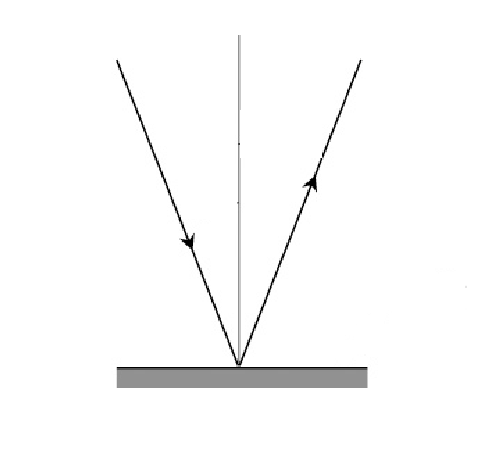
\includegraphics[width=2in]{particle_collision.png}
  \caption{\label{fig:collision-angle}Mechanics of a Billiard Ball Colliding with a Table Edge}
\end{figure}

Now, we shall label the horizontal sides of the table $h$ and the vertical sides of the table $v$. Whenever the billiard ball collides with a horizontal side (labelled $h$), we shall call the resulting collision an $h$-collision. Whenever the ball collides with a vertical side (labelled $v$), we shall call the resulting collision a $v$-collision.

We shall now define what this paper will be primarily interested in, a sequence of collisions:

\begin{definition}
  A \emph{collision sequence} ($\alpha$) is a sequence of $v$ and $h$ collisions which starts and ends with an $h$ collision for some ball $b$ with initial position $\bvec{x}_0$ and intial velocity $\bvec{v}_0$.
\end{definition}

Notice that all non-trivial initial conditions for a billiard ball will result in infinitely many $h$-collisions. The only initial conditions for which this is not true are when the initial velocity is parallel to the horizontal ($\bvec{v}_0 = (1, 0)$) so that the ball bounces infinitely between the two vertical sides. The proof of this is trivial and should become clear once the tiling representation is presented, so we will omit it.

Thus, it is perfectly reasonable to constrain a ball's collision sequence to begin and end with an $h$ collision, since one simply needs to extend the number of collisions one watches until the sequence of collisions begins and ends with an $h$-collision. This constraint will later make it easier to reason about properties of sequences.

\subsection{Example Collision Sequence}

To understand collision sequences better, we shall provide an example. Consider a billiard ball with intial position $\bvec{x}_0 = (0.75, 0.75)$ and initial velocity $\bvec{v}_0 = (0.23, 0.05)$.

\begin{figure}
  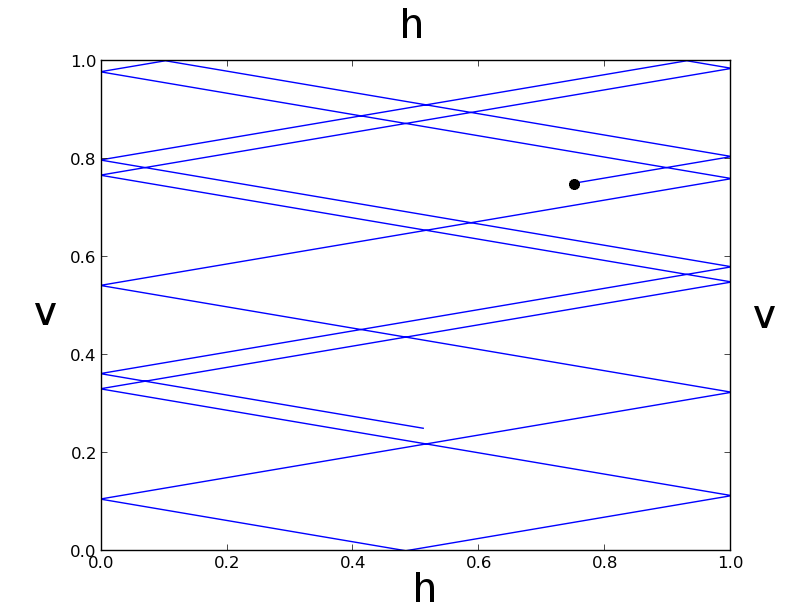
\includegraphics[width=2in]{example.png}
  \caption{\label{fig:example}Example Billiard Ball Trajectory, $x_0 = (0.75, 0.75)$, $v_0 = (0.23, 0.05)$}
\end{figure}

We can see from the figure that the collisions that it makes, denoting a $v$-collision with a $v$ and an $h$-collision with an $h$, are $\{v, h, v, v, v, v, v, h, v, v, v, v, v, h, v, v, v\}$. A valid collision sequence given these initial conditions would start and end with an $h$ collision. A possible example would be:

\begin{eqnarray}
  \alpha = hvvvvvhvvvvvh
\end{eqnarray}

Notice that the collisions will continue infinitely, so one could imagine extending this collision sequence to include more $v$ and $h$ collisions. Although not shown in the picture, the following collision sequence would also be valid if one continued showing the trajectory of the ball in future collisions:

\begin{eqnarray}
  \alpha = hvvvvvhvvvvvhvvvvvh
\end{eqnarray}

\subsection{Simplifications}

There are also a couple of simplifications that we can make without loss of generality that will make talking about billiard balls, their initial conditions, and their collision sequences easier.

\begin{itemize}
  \item We can change the magnitude of the initial velocity $\bvec{v}_0$ without changing any collision sequences. This is because only the direction of $\bvec{v}_0$ affects the points of collision of the billiard ball with the table. Thus, the only part of the initial velocity that we care about is the velocity's direction. We could alternatively talk about the angle $\gamma$ that $\bvec{v}_0$ makes with the positive horizontal line (just as in polar coordinates).
  \item We can constrain the initial velocity's angle to the range $\gamma \in [0, \pi/2]$. This is because any intial velocity in the range $\gamma \in [-\pi/2, \pi/2]$ will create equivalent collision sequences as $\pi + \gamma$ (this will be clear once we present the tiling representation later in the paper). Moreover, any angle in the range $\gamma \in [0, \pi/2]$ will create equivalent collision sequences as those in $[-\pi/2, 0]$ by simply reflecting the cube about one of its horizontal sides.
\end{itemize}

Using these simplifications, we will constrain the initial conditions of all billiard balls throughout the rest of the paper so that the initial velocity $\bvec{v}_0$ has an angle $\gamma \in [0, \pi/2]$.
